\PassOptionsToPackage{unicode=true}{hyperref} % options for packages loaded elsewhere
\PassOptionsToPackage{hyphens}{url}
\PassOptionsToPackage{dvipsnames,svgnames*,x11names*}{xcolor}
%
\documentclass[10pt,ignorenonframetext,]{beamer}
\usepackage{pgfpages}
\setbeamertemplate{caption}[numbered]
\setbeamertemplate{caption label separator}{: }
\setbeamercolor{caption name}{fg=normal text.fg}
\beamertemplatenavigationsymbolsempty
% Prevent slide breaks in the middle of a paragraph:
\widowpenalties 1 10000
\raggedbottom
\setbeamertemplate{part page}{
\centering
\begin{beamercolorbox}[sep=16pt,center]{part title}
  \usebeamerfont{part title}\insertpart\par
\end{beamercolorbox}
}
\setbeamertemplate{section page}{
\centering
\begin{beamercolorbox}[sep=12pt,center]{part title}
  \usebeamerfont{section title}\insertsection\par
\end{beamercolorbox}
}
\setbeamertemplate{subsection page}{
\centering
\begin{beamercolorbox}[sep=8pt,center]{part title}
  \usebeamerfont{subsection title}\insertsubsection\par
\end{beamercolorbox}
}
\AtBeginPart{
  \frame{\partpage}
}
\AtBeginSection{
  \ifbibliography
  \else
    \frame{\sectionpage}
  \fi
}
\AtBeginSubsection{
  \frame{\subsectionpage}
}
\usepackage{lmodern}
\usepackage{amssymb,amsmath}
\usepackage{ifxetex,ifluatex}
\usepackage{fixltx2e} % provides \textsubscript
\ifnum 0\ifxetex 1\fi\ifluatex 1\fi=0 % if pdftex
  \usepackage[T1]{fontenc}
  \usepackage[utf8]{inputenc}
  \usepackage{textcomp} % provides euro and other symbols
\else % if luatex or xelatex
  \usepackage{unicode-math}
  \defaultfontfeatures{Ligatures=TeX,Scale=MatchLowercase}
\fi
\usetheme[]{Singapore}
\usefonttheme{serif}
% use upquote if available, for straight quotes in verbatim environments
\IfFileExists{upquote.sty}{\usepackage{upquote}}{}
% use microtype if available
\IfFileExists{microtype.sty}{%
\usepackage[]{microtype}
\UseMicrotypeSet[protrusion]{basicmath} % disable protrusion for tt fonts
}{}
\IfFileExists{parskip.sty}{%
\usepackage{parskip}
}{% else
\setlength{\parindent}{0pt}
\setlength{\parskip}{6pt plus 2pt minus 1pt}
}
\usepackage{xcolor}
\usepackage{hyperref}
\hypersetup{
            pdftitle={Module 4: Classification},
            pdfauthor={Stefanie Muff, Institutt for matematiske fag},
            colorlinks=true,
            linkcolor=Maroon,
            filecolor=Maroon,
            citecolor=Blue,
            urlcolor=blue,
            breaklinks=true}
\urlstyle{same}  % don't use monospace font for urls
\newif\ifbibliography
\usepackage{graphicx,grffile}
\makeatletter
\def\maxwidth{\ifdim\Gin@nat@width>\linewidth\linewidth\else\Gin@nat@width\fi}
\def\maxheight{\ifdim\Gin@nat@height>\textheight\textheight\else\Gin@nat@height\fi}
\makeatother
% Scale images if necessary, so that they will not overflow the page
% margins by default, and it is still possible to overwrite the defaults
% using explicit options in \includegraphics[width, height, ...]{}
\setkeys{Gin}{width=\maxwidth,height=\maxheight,keepaspectratio}
\setlength{\emergencystretch}{3em}  % prevent overfull lines
\providecommand{\tightlist}{%
  \setlength{\itemsep}{0pt}\setlength{\parskip}{0pt}}
\setcounter{secnumdepth}{0}

% set default figure placement to htbp
\makeatletter
\def\fps@figure{htbp}
\makeatother

\usepackage{multicol}

\title{Module 4: Classification}
\providecommand{\subtitle}[1]{}
\subtitle{ISTx1003 Statistisk læring og Data Science}
\author{Stefanie Muff, Institutt for matematiske fag}
\date{November xy, 2021}

\begin{document}
\frame{\titlepage}

\begin{frame}{Plan for i dag}
\protect\hypertarget{plan-for-i-dag}{}

\(~\)

\begin{itemize}
\item
  Læringsmål og ressurser
\item
  Hva er klassifikasjon
\item
  Trening, validering og testing (3 datasett)
\item
  \(k\)-nærmeste nabo (kNN): en intuitiv metode
\item
  Forvirringsmatrise og feilrate for å evaluere metoden
\item
  Logistisk regresjon
\end{itemize}

\end{frame}

\begin{frame}{Læringsmål}
\protect\hypertarget{luxe6ringsmuxe5l}{}

\begin{itemize}
\item
  kunne forstå hva klassifikasjon går ut på og kjenne situasjoner der
  klassifikasjon vil være en aktuell metode å bruke
\item
  kjenne begrepene treningssett, valideringssett og testsett og forstå
  hvorfor vi lager dem og hva de skal brukes til
\item
  vite hva en forvirringsmatrise er, og kjenne til begrepene feilrate og
  nøyaktighet (accuracy)
\item
  forstå tankegangen bak \(k\)-nærmeste nabo-klassifikasjon, valg av k
\item
  kjenne til modellen for logistisk regresjon, og kunne tolke de
  estimerte koeffisientene
\item
  forstå hvordan vi utfører klassifikasjon i Python
\item
  kunne besvare oppgave 2 av prosjektoppgaven
\end{itemize}

\end{frame}

\begin{frame}{Læringsressurser}
\protect\hypertarget{luxe6ringsressurser}{}

\vspace{2mm}

\vspace{2mm}

\begin{itemize}
\item
  \textbf{Kompendium}: Klassifikasjon (pdf og html, by Mette Langaas)
\item
  \textbf{Korte videoer}: (by Mette Langaas)

  \begin{itemize}
  \tightlist
  \item
    Introduksjon og \(k\)-nærmeste nabo klassifiiasjon (10:58)
  \item
    Logistisk regresjon (14:17)
  \end{itemize}
\item
  \textbf{Disse slides} med notater
\end{itemize}

\end{frame}

\begin{frame}{Klassifikasjon -- hva er det?}
\protect\hypertarget{klassifikasjon-hva-er-det}{}

\begin{itemize}
\item
  Mål:

  \begin{itemize}
  \item
    tilordne en ny observasjon til en av flere \emph{kjente} klasser
  \item
    lage en klassifikasjonsregel
  \item
    estimere sannsynligheten for at en ny observasjon tilhører de ulike
    klassene
  \end{itemize}
\end{itemize}

\vspace{2mm}

For hver av de uavhengige observasjonene \(i=1,\ldots,n\) har vi

\begin{itemize}
\tightlist
\item
  Forklaringsvariabler \((x_{1i},x_{2i},\ldots,x_{pi})\)
\item
  En kategorisk responsvariablel \(y_i\).
\end{itemize}

\end{frame}

\begin{frame}

\begin{block}{Eksempler}

\vspace{2mm}

\begin{itemize}
\tightlist
\item
  Hvilke tall er handskrevet på brev? Og hva er sannsynligheten for de
  ulike tallene (=klasser). 
\end{itemize}

\centering

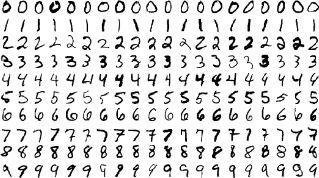
\includegraphics[width=0.5\textwidth,height=\textheight]{mnist.jpeg}

\vspace{2mm}

\flushleft

\begin{itemize}
\tightlist
\item
  ``Spam eller ham?'' spam filer: Klassifikasjon om en e-post er spam
  eller ikke.\\
  Binær: Respons variable er ``ja''/``nei'' (1/0).
\end{itemize}

\vspace{2mm}

\begin{itemize}
\tightlist
\item
  Kommer en gitt kunde til å betale tilbake lånet sitt?
\end{itemize}

\vspace{2mm}

\begin{itemize}
\tightlist
\item
  Prognose om noen blir syk (hjertesykdom, kreft\ldots{}) og
  sannsynligheten for det.
\end{itemize}

\end{block}

\end{frame}

\begin{frame}

Noe om tilsvarende oppgave i prosjektet

\end{frame}

\begin{frame}

\begin{block}{Syntetisk eksempel}

\(~\)

\begin{itemize}
\tightlist
\item
  Et datasett med folgende struktur: \((x_{1i},x_{2i},y_i)\).
  \vspace{2mm}
\end{itemize}

\begin{center}\includegraphics[width=0.6\linewidth]{2Klassifikasjon_files/figure-beamer/unnamed-chunk-1-1} \end{center}

Spørsmål vi vil besvar: Hva vil beste klassifikasjonsgrense være?

\end{block}

\end{frame}

\begin{frame}

\begin{block}{Et eksempel til}

\end{block}

\end{frame}

\begin{frame}{Data}
\protect\hypertarget{data}{}

\vspace{2mm}

Datasett: \((x_{1i},x_{2i},\ldots, x_{pi},y_i)\)

\vspace{2mm}

Vi må dele datasettet i tre deler:

\vspace{2mm}

\begin{itemize}
\tightlist
\item
  Treningsdata
\item
  Valideringsdata
\item
  Testdata
\end{itemize}

\vspace{5mm}


\includegraphics{datasett.png}

\vspace{2mm}

Hvorfor det?

\end{frame}

\begin{frame}{Trening-, validering- og testsett for syntetiske data}
\protect\hypertarget{trening--validering--og-testsett-for-syntetiske-data}{}

\begin{center}\includegraphics[width=0.9\linewidth]{2Klassifikasjon_files/figure-beamer/unnamed-chunk-2-1} \end{center}

\end{frame}

\begin{frame}{\(k\)-nærmeste-nabo-klassifikasjon}
\protect\hypertarget{k-nuxe6rmeste-nabo-klassifikasjon}{}

For å finne klassifikasjonsreglen bruker vi bare treningsdataene.

Bruker bare treningsdataene. Algoritmen:

\begin{enumerate}
[1)]
\item
  Ny observasjon: \(x_0=(x_{1,0}, x_{2,0} , \ldots , x_{p,0})\) .
  Hvilken klasse bør denne klassifiseres til?
\item
  Finn de \(k\) nærmeste naboene til observasjonen i treningssettet.
\item
  Sannsynligheten for at den nye observasjonen tilhører klasse 1 anslår
  vi er andelen av de k nærmeste naboene som har tilhører klasse 1.
  Ditto for de andre klassene.
\item
  Klassen til den nye observasjonen er den som har størst sannsynlighet.
  Det blir det samme som å bruke flertallsavstemming.
\end{enumerate}

\end{frame}

\begin{frame}{\(k\)-nærmeste-nabo-klassifikasjon}
\protect\hypertarget{k-nuxe6rmeste-nabo-klassifikasjon-1}{}

\vspace{5mm}

Tre sp\oe rsm\aa l: \vspace{5mm}

\begin{itemize}
\tightlist
\item
  Hva betyr ``n\ae rmest''? Vi trenger en definision av avstand.
\end{itemize}

\vspace{1.5cm}

\begin{itemize}
\tightlist
\item
  Hvilke verdier kan \(k\) ha?
\end{itemize}

\vspace{1.5cm}

\begin{itemize}
\tightlist
\item
  Hvordan bestemmer vi \(k\)?
\end{itemize}

\end{frame}

\begin{frame}

\begin{block}{Hva betyr nærmest?}

\vspace{2mm}

Nærmest er definert ved å bruke euklidsk avstand.

\centering

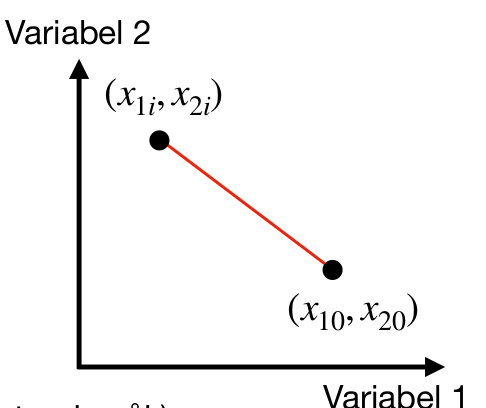
\includegraphics[width=0.4\textwidth,height=\textheight]{avstand.png}

\flushleft

Euklidsk avstand: \[D_E(i,0)=\sqrt{\sum_{j=1}^p (x_{ji}-x_{j0})^2 }\]

Andre avstandsm\aa l kan ogs\aa  ~brukes, men Euklidsk avstand er mest
vanlig.

\end{block}

\end{frame}

\begin{frame}

\begin{block}{N\ae rmeste naboer}

\vspace{5mm}

\begin{center}\includegraphics[width=0.6\linewidth]{2Klassifikasjon_files/figure-beamer/unnamed-chunk-3-1} \end{center}

\end{block}

\end{frame}

\begin{frame}

\begin{block}{N\ae rmeste naboer}

\vspace{5mm}

\begin{center}\includegraphics[width=0.6\linewidth]{2Klassifikasjon_files/figure-beamer/unnamed-chunk-4-1} \end{center}

\end{block}

\end{frame}

\begin{frame}

\begin{block}{Tegn klassegrenser}

\vspace{5mm}

\begin{center}\includegraphics[width=0.6\linewidth]{2Klassifikasjon_files/figure-beamer/unnamed-chunk-5-1} \end{center}

\end{block}

\end{frame}

\begin{frame}

\begin{block}{Hvordan ser klassegrensene ut?}

\(~\)

Husk: Vi bruker treningssettet for å finne klassifikasjonsreglen:

\(~\)

\begin{center}\includegraphics[width=0.7\linewidth]{2Klassifikasjon_files/figure-beamer/unnamed-chunk-6-1} \end{center}

\end{block}

\end{frame}

\begin{frame}

\begin{block}{Hvordan ser klassegrensene ut?}

\(~\) Svar: It depends!

\begin{center}\includegraphics[width=0.7\linewidth]{2Klassifikasjon_files/figure-beamer/knnplot-1} \end{center}

\end{block}

\end{frame}

\begin{frame}

\begin{block}{Men vent\ldots{} hvordan velger vi \(k\) da?}

\(~\)

Vi så jo at

\begin{itemize}
\tightlist
\item
  Vi skal ikke velge \(k\) for liten, ellers blir grensen for fleksibel.
\end{itemize}

\(~\)

Men:

\begin{itemize}
\tightlist
\item
  Vi skal antakeligvis heller ikke velge \(k\) for stor, ellers kan bli
  for ufleksibel.
\end{itemize}

\(~\)

Det er noe som kalles en trade-off, og vi skal bruk valideringssettet
for få en ide om kvaliteten i klassifikasjonen.

\end{block}

\end{frame}

\begin{frame}

\begin{block}{Forvirringsmatrise}

Forvirringsmatrise med to klasser:

\vspace{4cm}

\begin{itemize}
\tightlist
\item
  \textbf{Feilrate}: andel feilklassifiserte observasjoner.
\end{itemize}

\(~\)

\centering

Derfor: Vi velger den \(k\) som minimerer feilraten på
\emph{valideringssettet} (ikke trainingssettet!).

\end{block}

\end{frame}

\begin{frame}

Marker og tell antall gale klassifiseringer på valideringssettet
(\(k=1\)):

\begin{center}\includegraphics[width=0.7\linewidth]{2Klassifikasjon_files/figure-beamer/knnplot2-1} \end{center}

\end{frame}

\begin{frame}

Igjen, men nå med \(k=99\):

\begin{center}\includegraphics[width=0.7\linewidth]{2Klassifikasjon_files/figure-beamer/knnplot3-1} \end{center}

\end{frame}

\begin{frame}

\begin{block}{Feilrate i valideringssettet}

\(~\)

Det kan nå gjøres med alle \(k=1,3,\ldots\), \(k\leq n\). De ser slik
ut:

\vspace{5mm}

\begin{center}\includegraphics[width=0.7\linewidth]{2Klassifikasjon_files/figure-beamer/knn_validation-1} \end{center}

\end{block}

\end{frame}

\begin{frame}

Klassegrensene ser ganske likt ut for \(k=15\) og \(k=99\):

\begin{center}\includegraphics[width=0.7\linewidth]{2Klassifikasjon_files/figure-beamer/knnplot4-1} \end{center}

\end{frame}

\begin{frame}{Data}
\protect\hypertarget{data-1}{}

\vspace{2mm}

Husk at vi hadde tre deler i datasettet:

\vspace{2mm}

\begin{itemize}
\tightlist
\item
  Treningssett: For å lage en klassifikasjonsregel
\item
  Valideringssett: For å finne på optimale hyperparametere
\item
  Testsett: For å evaluere regelen på fremtidige data
\end{itemize}

\vspace{5mm}


\includegraphics{datasett.png}

\vspace{2mm}

Nå kan vi bruk testsettet for å finne feilraten.

\end{frame}

\begin{frame}

Feilraten på testsettet for KNN med \(k=15\) (egentlig er \(k=31\) best,
men det gjør ikke en stor forskjell):

\begin{center}\includegraphics[width=0.6\linewidth]{2Klassifikasjon_files/figure-beamer/knnplot5-1} \end{center}

Feilraten er 0.09.

\end{frame}

\begin{frame}{\(k\)-nærmeste nabo klassifikasjon i Python}
\protect\hypertarget{k-nuxe6rmeste-nabo-klassifikasjon-i-python}{}

knaboer = np.arange(1,199,step=2)

val\_feilrate = np.empty(len(knaboer)) for i,k in enumerate(knaboer):
knn = KNeighborsClassifier(n\_neighbors=k,p=2)
knn.fit(df\_tren{[}{[}`x1',`x2'{]}{]}, df\_tren{[}`y'{]})
val\_feilrate{[}i{]} = 1-knn.score(df\_val{[}{[}`x1',`x2'{]}{]},
df\_val{[}`y'{]})

\end{frame}

\begin{frame}{Todo (adapt to the code they need in oppgave 2)}
\protect\hypertarget{todo-adapt-to-the-code-they-need-in-oppgave-2}{}

Plott feilrate:

plt.title(`k-NN for ulike verdier av antall naboer k') plt.plot(knaboer,
val\_feilrate, label=`Feilrate på valideringssettet') plt.xlabel(`Antall
naboer k'); plt.ylabel(`Feilrate') plt.show()

Velg k: mink\_valfeilrate = knaboer{[}np.where(val\_feilrate ==
val\_feilrate.min()){]} print(mink\_valfeilrate{[}0{]})

Sett opp klassifikator:

bestek=99 knn = KNeighborsClassifier(n\_neighbors=bestek,p=2)

Feilrate på testsett: knn.fit(df\_tren{[}{[}`x1',`x2'{]}{]},
df\_tren{[}`y'{]}) print(``Feilrate kNN:'', 1-
knn.score(df\_test{[}{[}`x1',`x2'{]}{]}, df\_test{[}`y'{]}))

\end{frame}

\begin{frame}

\begin{block}{Pensum for oppgave 2 -- hvor er vi nå?}

\begin{multicols}{2}
\begin{itemize}
\item trening/validering/test
\item hvorfor
\item hvordan bruke
\item viktig å tenke på
\end{itemize}

\vspace{4mm}

\begin{itemize}
\item tolke plott
\item boksplott histogram
\item kryssplott korrelasjon
\item hva ser vi etter når vi vil lage en god klassifikasjonsregel?
\end{itemize}

\vspace{15mm}

\begin{itemize}
\item Forvirringsmatrise og feilrate
\item evaluere modell
\item velg mellom to modeller eller metoder
\item velge hyperparameter
\end{itemize}

\vspace{4mm}

\begin{itemize}
\item $k$-nærmeste nabo (kNN)
\item forstå metoden
\item velge $k$
\end{itemize}

\vspace{4mm}

\begin{itemize}
\item logistisk regresjon
\item tolke estimerte koeffisienter
\item hypotesetest og p-verdi
\item velge mellom modeller
\end{itemize}
\end{multicols}

\end{block}

\end{frame}

\begin{frame}{Plan for i dag}
\protect\hypertarget{plan-for-i-dag-1}{}

\(~\)

\begin{itemize}
\item
  Læringsmål og ressurser
\item
  Hva er klassifikasjon
\item
  Trening, validering og testing (3 datasett)
\item
  \(k\)-nærmeste nabo (kNN): en intuitiv metode
\item
  Forvirringsmatrise og feilrate for å evaluere metoden
\item
  Logistisk regresjon
\end{itemize}

\end{frame}

\begin{frame}{Logistisk regresjon}
\protect\hypertarget{logistisk-regresjon}{}

\(~\)

\begin{itemize}
\tightlist
\item
  Kan bare handtere \emph{to klasser} \(y_i \in \{0,1\}\).
\end{itemize}

\(~\)

\begin{itemize}
\tightlist
\item
  Vi antar at \(Y_i\) har en \textbf{Bernoulli fordeling} med
  suksessannsynlighet \(p_i\), derfor:
\end{itemize}

\[y_i = \begin{cases} 1 \text{ med sannsynlighet } p_i, \\ 0 \text{ med sannsynlighet } 1-p_i. \end{cases}\]

\(~\)

\begin{itemize}
\tightlist
\item
  \textbf{Mål}: For forklaringsvariabler
  \((x_{1i},x_{2i},\ldots,x_{pi})\) vi vil estimere
  \(p_i = \text{Pr}(y_i=1 \mid x_1,\ldots,x_p)\).
\end{itemize}

\end{frame}

\begin{frame}[fragile]

\begin{block}{Eksempel: Kredittkort data}

\vspace{2mm}

Datasettet \texttt{Default} er tatt fra her:
\url{https://rdrr.io/cran/ISLR/man/Credit.html}

\vspace{2mm}

\textbf{Mål} : forutsi om en person ikke betaler kredittkortregning
(``person defaults''), avhengig av årsinntekten (income) og balansen på
kredittkortet (balance).

\textcolor{orange}{Orange: default=yes},
\textcolor{blue}{blue: default=no}.

\centering
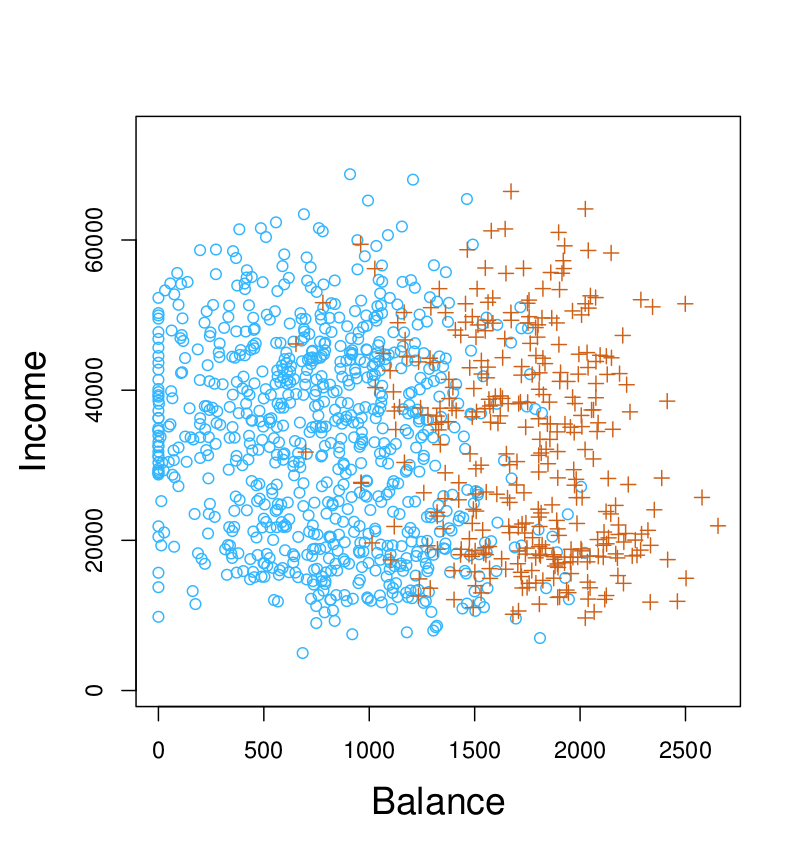
\includegraphics[width=0.5\textwidth,height=\textheight]{4.1a.png}

\end{block}

\end{frame}

\begin{frame}

Det ser ut som at ``Balance'' er en ganske go forklarende variabel til
Default (nei/ja).

\begin{center}\includegraphics[width=0.9\linewidth]{2Klassifikasjon_files/figure-beamer/unnamed-chunk-8-1} \end{center}

\end{frame}

\begin{frame}[fragile]

\begin{block}{Kan vi bare bruke linear regresjon for binær
klassifikasjon?}

\vspace{1mm}

For en binær responsvariabel \(Y =\) \texttt{yes} or \texttt{no}, og
forklaringsvariabler \(X\) bruker vi vannligvis en \emph{dummy encoding}
:

\[Y = \left\{ \begin{array}{ll}
0 & \text{if } \texttt{no} \ , \\
1 & \text{if } \texttt{yes} \ .
\end{array} \right.\]

\vspace{6mm}

\begin{center}\includegraphics[width=0.6\linewidth]{2Klassifikasjon_files/figure-beamer/unnamed-chunk-9-1} \end{center}

\end{block}

\end{frame}

\begin{frame}

\begin{itemize}
\item
  Kunne vi da ikke bare formulere en linear regresjonsmodell for \(X\)
  vs. \(Y\)?
\item
  Vi kunne jo klassifisere response som ``ja'' (1) hvis
  \(\hat{Y}> 0.5\).
\end{itemize}

\vspace{2mm}

\begin{itemize}
\tightlist
\item
  Problemet med linear regresjon: Vi kan forutsi \(Y<0\) eller \(Y>1\)
  med modellen, men en sannsynlighet er alltid mellom 0 og 1.
\end{itemize}

\(~\)

For kredittortdatasettet:

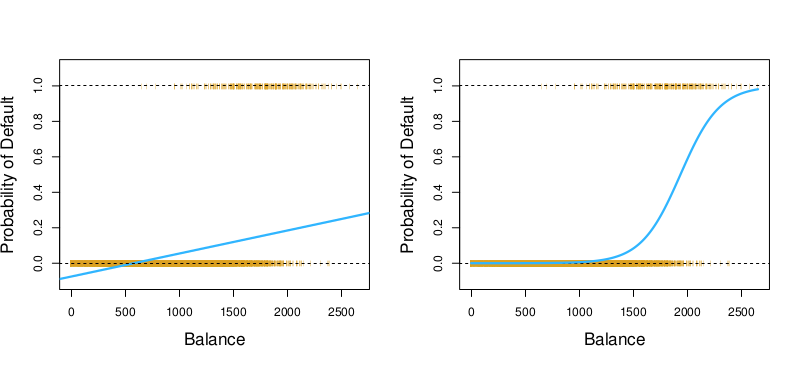
\includegraphics{4.2.png}

\end{frame}

\begin{frame}

\begin{block}{Vi trenger logistisk regresjon!}

\(~\)

\begin{center}\includegraphics[width=0.8\linewidth]{2Klassifikasjon_files/figure-beamer/unnamed-chunk-10-1} \end{center}

\end{block}

\end{frame}

\begin{frame}

\begin{block}{Enkel logistisk regresjon}

\(~\)

\begin{itemize}
\tightlist
\item
  Vi antar at responsen \(Y_i\) er binomisk fordelt med
  suksessannsynlighet \(p_i\)
\end{itemize}

\(~\)

\begin{itemize}
\tightlist
\item
  \textbf{Ideen}: å koble \(p_i\) sammen med forklaringsvariablen med en
  logistisk funksjon:
\end{itemize}

\[p_i = \frac{\exp(\beta_0 + \beta_x x_{1i}}{1+ \exp(\beta_0 + \beta_x x_{1i}} \]

\end{block}

\end{frame}

\end{document}
